\documentclass[11pt]{article}
\title{ECO208 Textbook Notes \\ \small Macroeconomic Theory Summer 2018 }
\author{Tianyu Du}
\date{\today}

\usepackage{spikey}
\usepackage{graphicx}
\usepackage{float}
\usepackage{xcolor}

\begin{document}
	\maketitle
	\tableofcontents
	
	\section{Chapter 9 A Two-Period Model: \\ The Consumption-Savings Decision and Credit Markets}
	
	\subsection{A Two-Period Model of the Economy}
	
	\subsubsection{Consumers}
	
	\paragraph{} There are $m$ consumers receiving exogenous income $y$. Incomes can be different for different consumers but all consumers pay the same lump sum tax $t$. Let $s$ denote saving and the \textbf{current period income constraint} for a typical consumer is
	
	\begin{equation}
		c + s = y - t
	\end{equation}
	
	\emph{Assumption: perfect credit market}
	\begin{assumption}
		All bonds in the credit market are indistinguishable and there is no risk associated with holding a bond.
	\end{assumption}
	\begin{assumption}
		Bonds are traded directly in the credit market without financial intermediaries.
	\end{assumption}
	\begin{assumption}
		The real rate of interest at which a consumer can lend is the same as the real rate of interest at which a consumer can borrow.
	\end{assumption}
	
	\paragraph{} There is no saving in the \emph{future period} (i.e. $s' \equiv 0$). The \textbf{future period income constraint} is 
	\begin{equation}
		c' = y' - t' + (1 + r)s
	\end{equation}
	By combining the income constraints in two period and the \textbf{lifetime budget constraint} can be characterized as 
	\begin{equation}
		c + \frac{c'}{1+r} = y - t + \frac{y' - t'}{1 + r}
	\end{equation}
	
	where the left hand side is the \textbf{present discounted value} of life time consumption and the right hand side captures the present discounted value of life time disposable income.
	\begin{definition}
		Define \textbf{lifetime wealth} $we$ as the present value of life time disposable income
		\[
			we := y - t + \frac{y' - t'}{1 + r}
		\]
	\end{definition}
	
	The life time income constraint can be rewrite as
	\begin{equation}
		c' = -(1+r)c + (1+r)we
	\end{equation}
	\begin{figure*}[h]
		\centering
		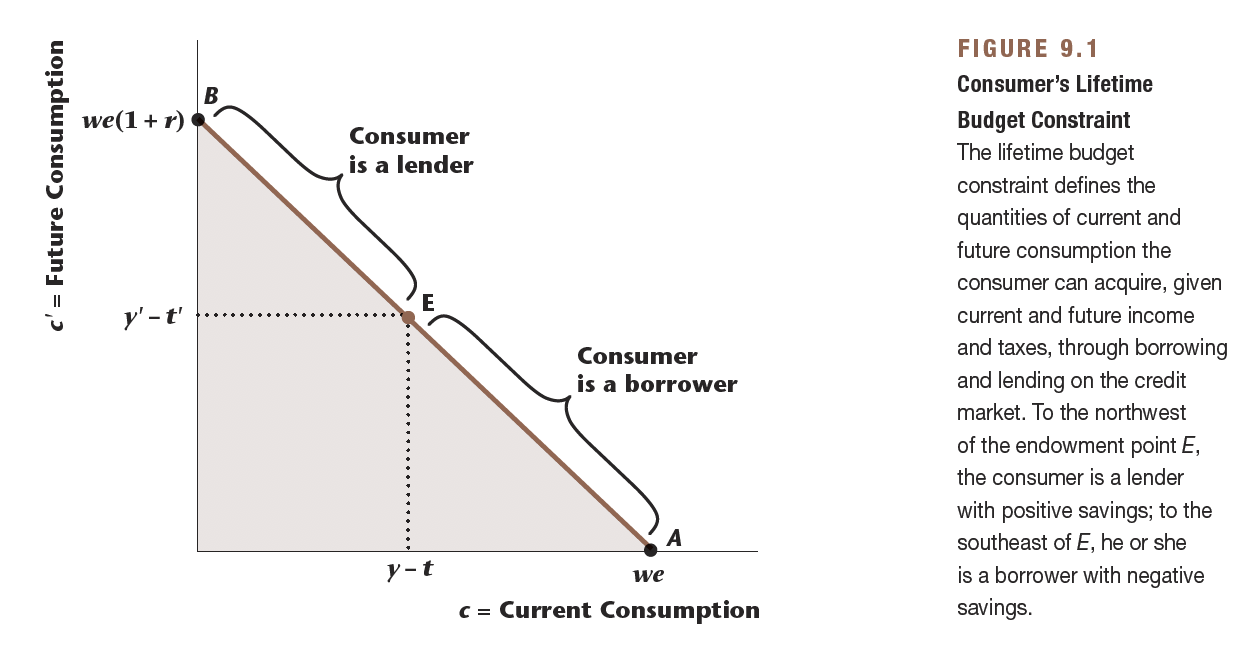
\includegraphics[width=\linewidth]{figures/91}
	\end{figure*}
	
	\newpage
	\begin{definition}
		\textbf{Endowment point} is the \textbf{consumption bundle} $(c, c')$ the consumer gets if he or she simply consumes disposable income in the current period and in the future period.
	\end{definition}
	
	\begin{assumption}
		We assume the consumers' preferences have three properties:
		\begin{enumerate}
			\item \textbf{Monotonicity} more is always preferred to less.
			\item \textbf{Convexity} the consumer likes diversity in his or her consumption bundle.
			\item Current consumption and future consumption are normal goods.
		\end{enumerate}
	\end{assumption}
	As figures below show, at the optimal point $A=(c^*, c'^*)$,
		\[
		MRS_{c, c'} = \frac{dc'}{dc} = -\frac{MU_c}{MU_{c'}}= 1 + r
		\]
	as it is on the tangency point.
	\begin{figure*}[h]
		\begin{minipage}{0.6\linewidth}
			\centering
			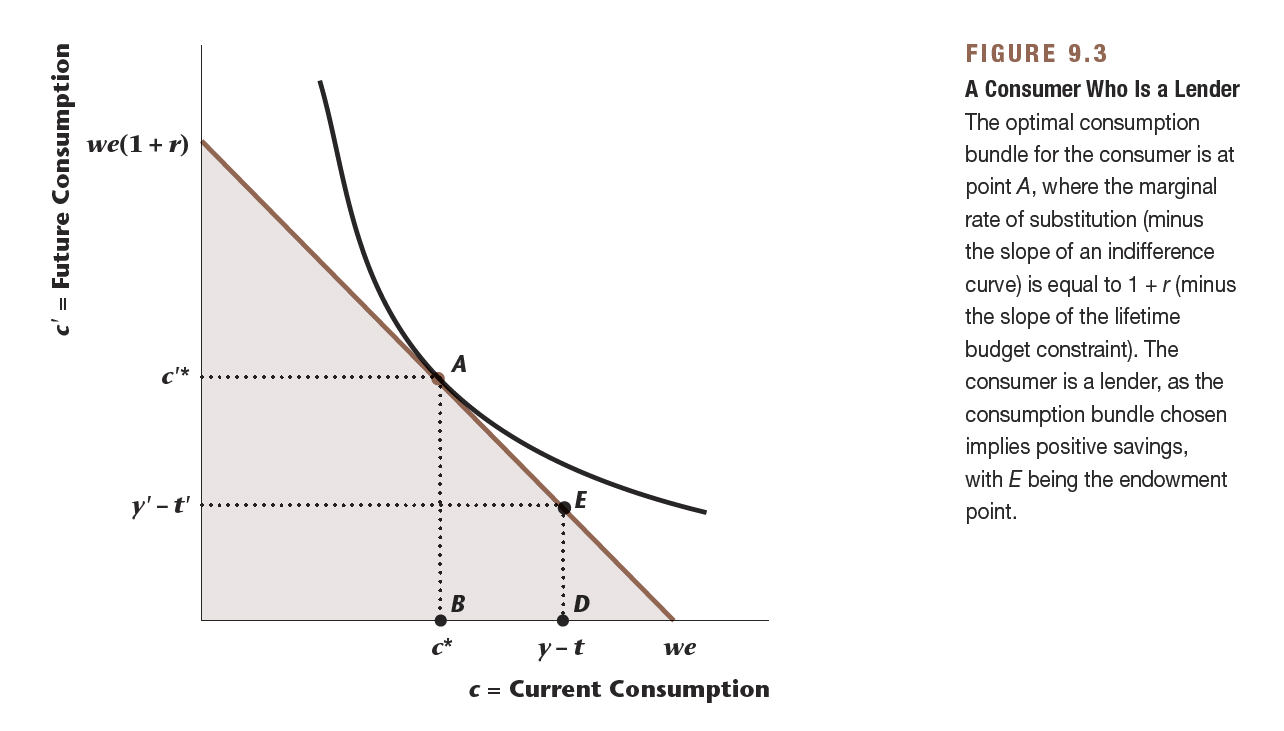
\includegraphics[width=\linewidth]{figures/93}
		\end{minipage}
		\begin{minipage}{0.6\linewidth}
			\centering
			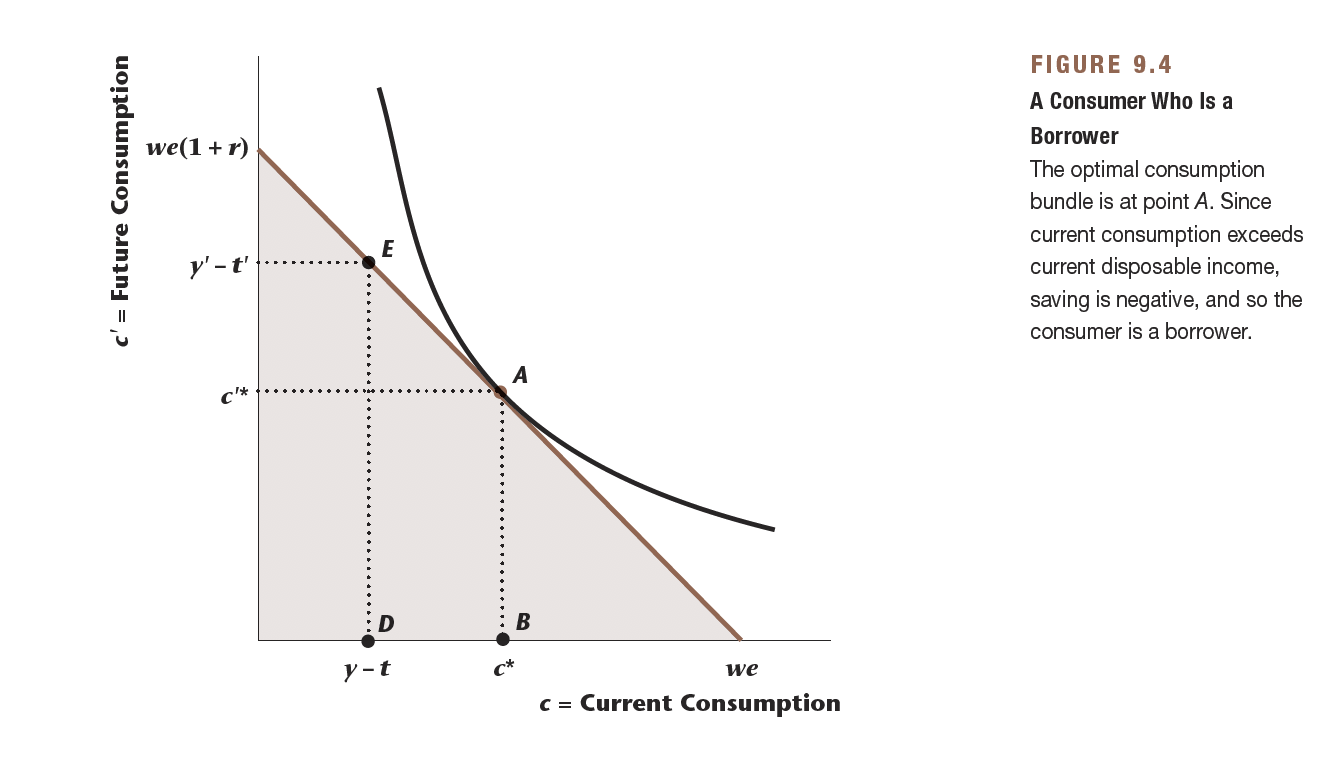
\includegraphics[width=\linewidth]{figures/94}
		\end{minipage}
	\end{figure*}
	
	\subsection{Experiments}
		\subsubsection{An Increase in Current-Period Income}
		\paragraph{Pure income effect} Increase in $we$ and parallel shifting on budget constraint. 
		\paragraph{Consumption Smoothing} As current income increases, the consumer wants to spread this additional income over both periods and not consume it all in the current period. Therefore
		\[
			\Delta y > \Delta c > 0\ and\ \Delta s > 0
		\]
		
		\begin{figure*}[h]
			\centering
			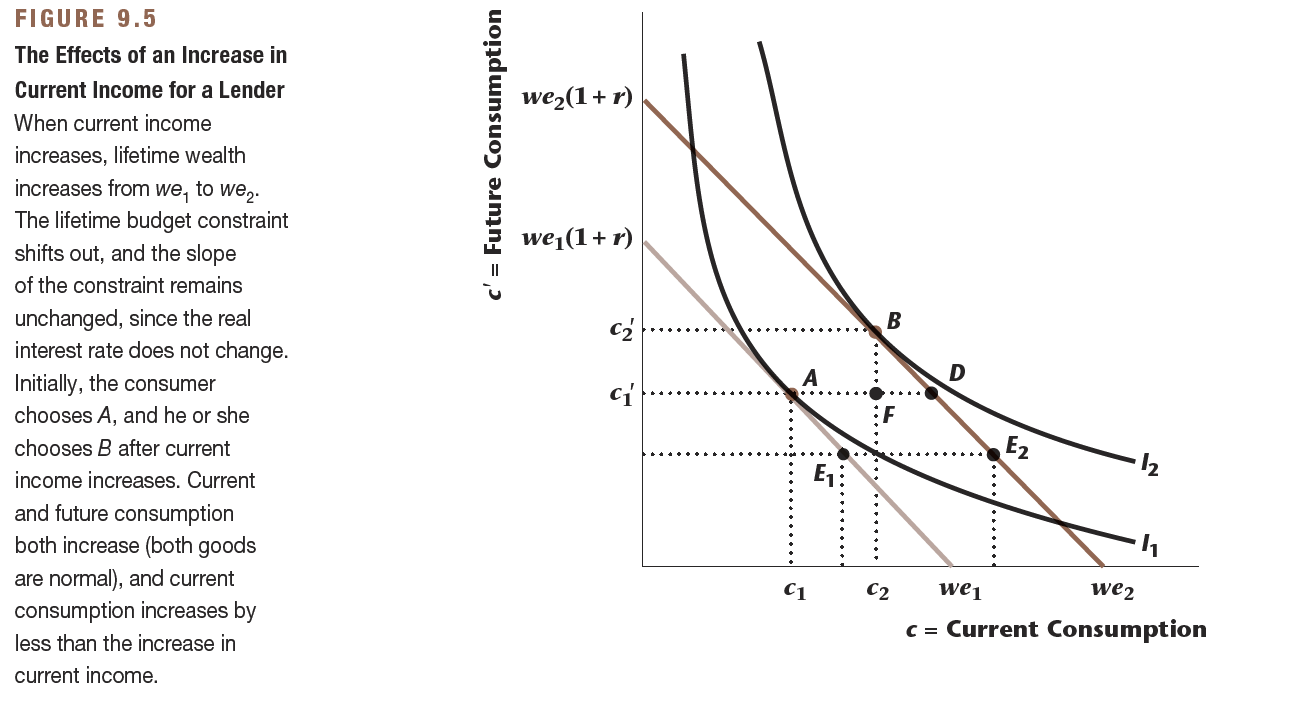
\includegraphics[width=\linewidth]{figures/95}
		\end{figure*}
		
		\paragraph{Excess variability} although consumption is smoother than income, as the theory predicts, consumption is not  quite smooth enough to tightly match the theory. The excess variability of aggregate consumption relative to aggregate income can be explained by 
		\begin{enumerate}
			\item \emph{There are imperfections in the credit market.}
			\item \emph{When all consumers are trying to smooth consumption in the same way simultaneously, this will change the market prices/ interest rate.}
		\end{enumerate}
		
		\subsubsection{An Increase in Future Income}
		\paragraph{Pure income effect} causes an out shifting of budget line and increases consumption in both periods. Due to backward consumption smoothing, even with $\Delta t = \Delta y = 0$,
		\[
			\Delta c > 0\ and\ \Delta s < 0
		\]
		\begin{figure*}[h]
			\centering
			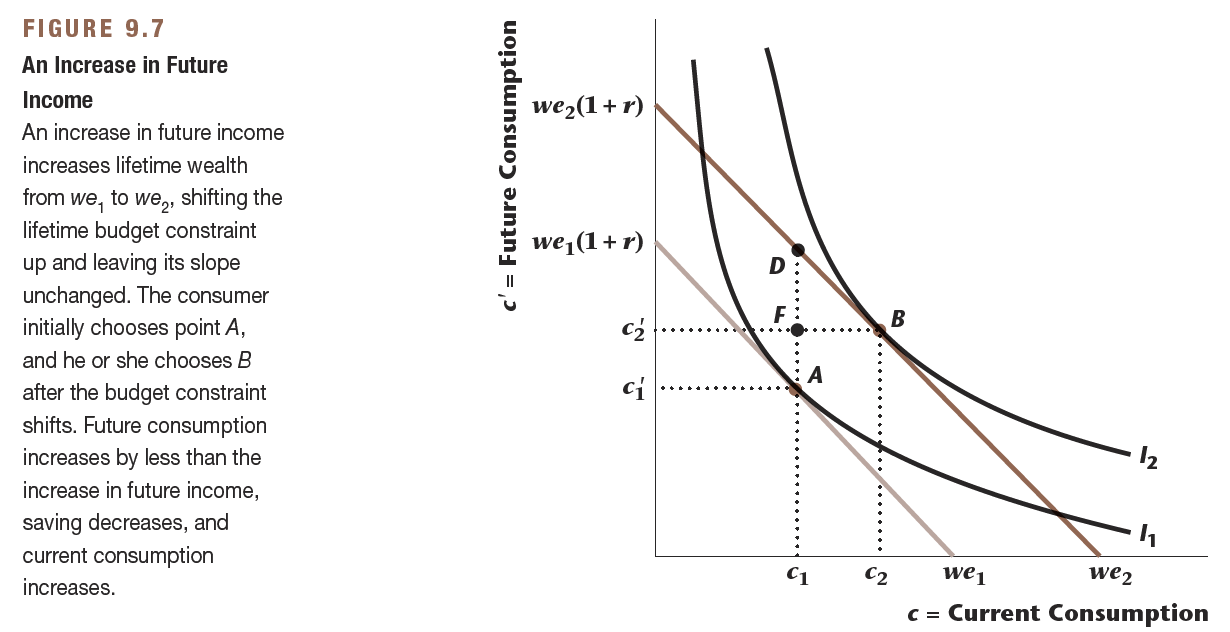
\includegraphics[width=\linewidth]{figures/97}
		\end{figure*}
		
		\newpage
		\subsubsection{Temporary and Permanent Changes in Income}
		\begin{definition}
			\textbf{Permanent income hypothesis} by Milton Friedman argued that a primary determinant of a consumer's current consumption is his or her \textbf{permanent income}.
		\end{definition}
		\par \emph{Temporary} changes in income yield small changes in permanent income (lifetime wealth) and therefore leads to a small effects on current consumption. Whereas \emph{permanent} changes in income have large effects on permanent income and current consumption.
		
		\begin{figure*}[h]
			\centering
			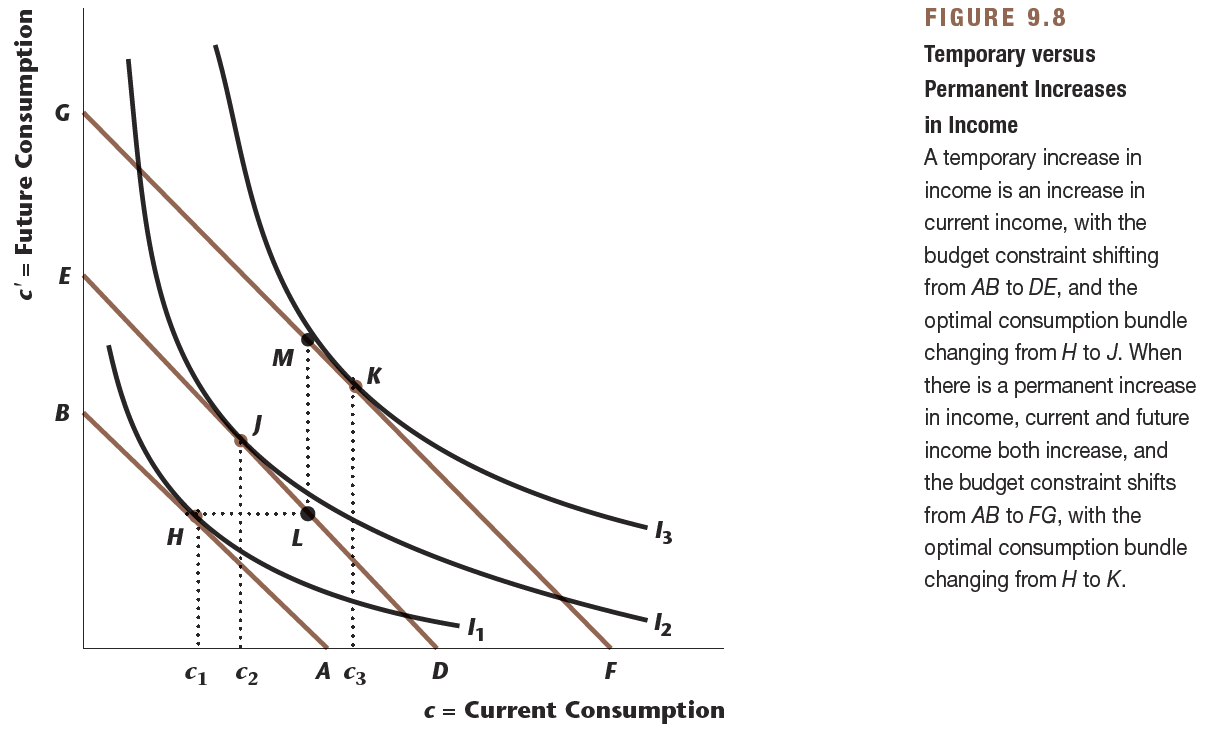
\includegraphics[width=\linewidth]{figures/98}
		\end{figure*}
		
		\newpage
		\subsubsection{An Increase in the Real Interest Rate}
		\paragraph{Effect} combined effect of both income effect and substitute effect.
		
		\begin{remark}
			the relative price of consumption goods in terms of current consumption goods is
			\[
				\frac{1}{1+r}
			\]
		\end{remark}
		
		\begin{remark}
			the effect on optimal $(c, c', s)$ would be different for lenders and borrowers.
		\end{remark}
		
		\paragraph{Lender} Consider an increase in real interest rate. For lenders, they intend to lend out current period income in exchange for future period consumption. Therefore, increase in return on saving would have a positive income effect on them.
		
		\begin{center}
			\begin{tabular}{l|ccc}
				Var & SE & IE & Total\\
				\hline
				$c$ & - & + & ?\\
				$c'$ & + & + & +\\
				$s$ & + & - & ? \\
			\end{tabular}
		\end{center}
		\begin{figure*}[h]
			\centering
			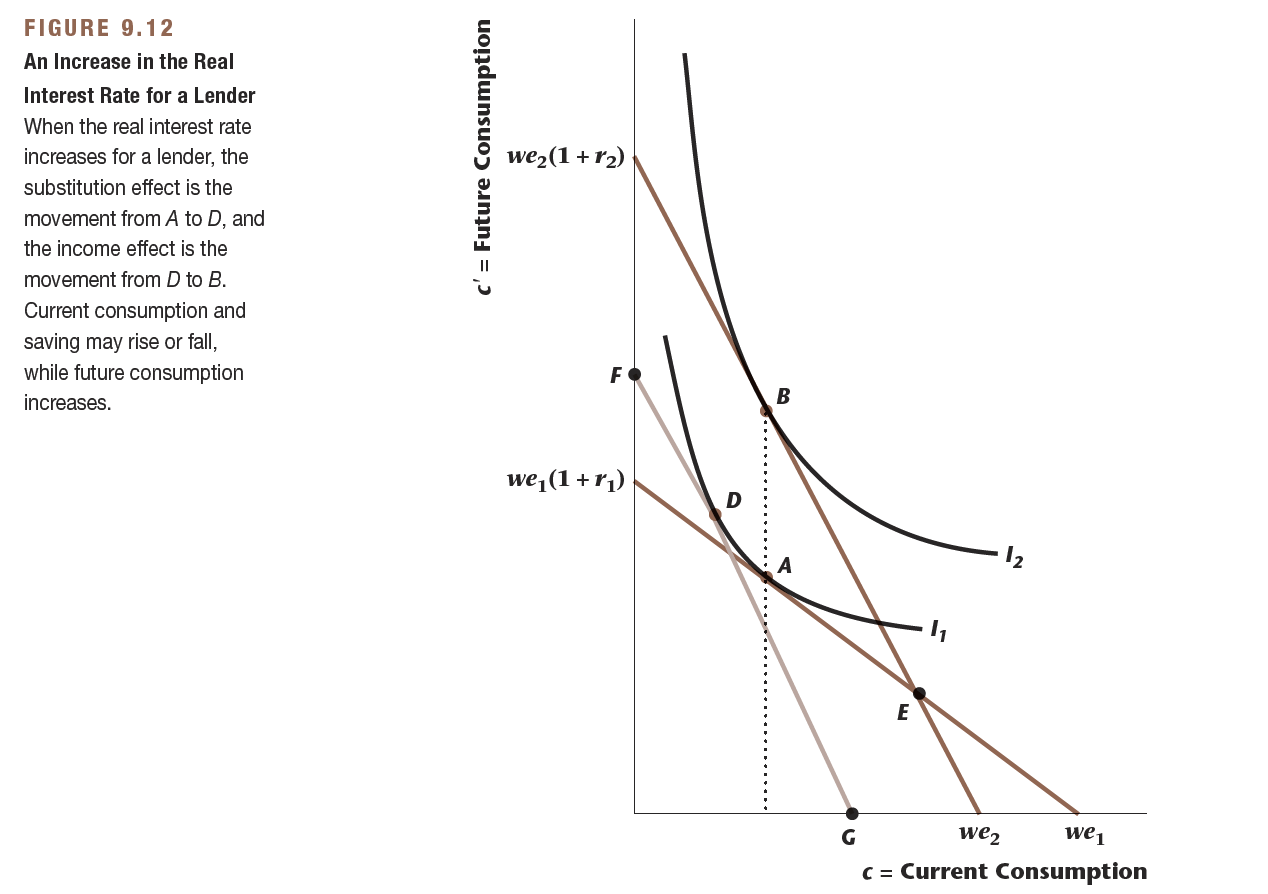
\includegraphics[width=\linewidth]{figures/912}
		\end{figure*}

		\newpage
		\paragraph{Borrowers} Consider an increase in real interest rate

		\begin{center}
			\begin{tabular}{l|ccc}
				Var & SE & IE & Total\\
				\hline
				$c$ & - & - & -\\
				$c'$ & + & - & ?\\
				$s$ & + & + & + \\
			\end{tabular}
		\end{center}
		
		\begin{figure*}[h]
			\centering
			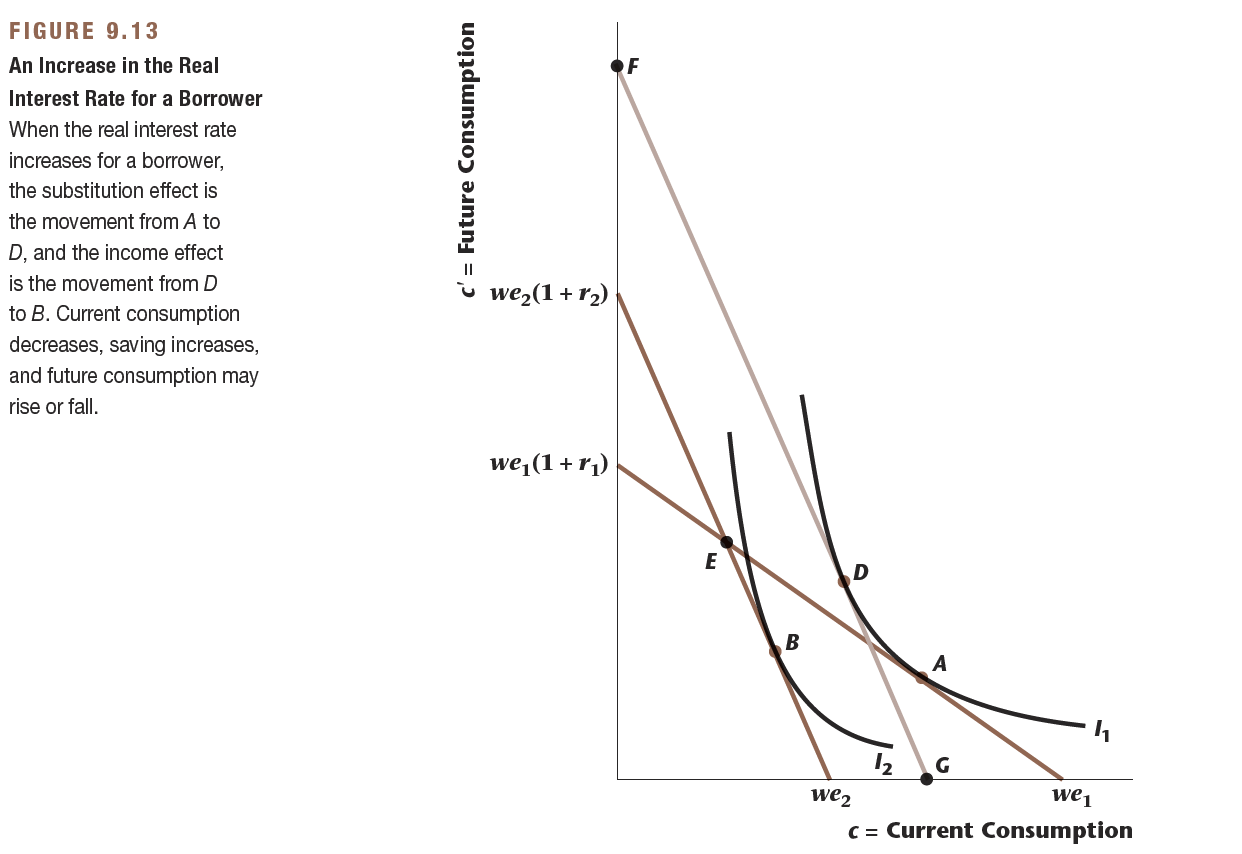
\includegraphics[width=\linewidth]{figures/913}
		\end{figure*}
		
		\begin{color}{blue}
		\begin{remark}
			For both borrower and lender, \emph{the substitution effects of change in real interest rate towards the same direction}. SE simply captures the change in relative price of current and future consumption ($\frac{1}{1+r}$). \emph{The income effects for borrower and lender work towards the opposite directions}.
		\end{remark}
		\end{color}
		
		\subsection{Government}
		
		\begin{assumption}
			Government bonds and private bonds are indistinguishable.
		\end{assumption}
		
		\par Let $T = mt$ denote the total tax collected by government. The \textbf{current period budget} for government is
		\begin{equation}
			G = T + B, \ B \in \R
		\end{equation}
		and the \textbf{future period budget} for government is
		\begin{equation}
			G' + (1+r)B = T'
		\end{equation}
		The \textbf{government present-value budget constraint} is
		\begin{equation}
		G + \frac{G'}{1 + r} = T + \frac{T'}{1 + r}
		\end{equation}
		
		\subsection{Competitive Equilibrium}
		\par Consumers and the government interact in the \textbf{credit market}. And in a competitive equilibrium, three conditions must hold:
		\begin{enumerate}
			\item Each consumer chooses $(c, c', s)$ optimally given the real interest rate $r$.
			\item Government present-value budget constraint, equation (7), holds.
			\item The credit market clears.
		\end{enumerate}
		Equivalently, let $\mc{I}$ be the collection of consumer indices,
		\[
		\begin{color}{red}
			\begin{cases}
				MRS_{c, c'}^{i} = 1+r\ \forall i \in \mc{I}\\
				G + \frac{G'}{1+r} = T + \frac{T'}{1+r} \\
				S^p = \sum_{i\in\mc{I}}{s_i} = B \\
			\end{cases}
		\end{color}
		\]
		On aggregate for consumers, 
		\begin{equation}
			S^p =  \sum_{i \in \mc{I}}{s_i} = \sum_{i \in \mc{I}}\big \{y_i - c_i - t \big \} = Y - C - T
		\end{equation}
		and by the second condition for competitive equilibrium and government's first period budget constraint, we have 
		\begin{equation}
			B = Y - C - T = G - T \implies \begin{color}{red} Y = C + G \end{color}
		\end{equation}
		
		\subsection{The Ricardian Equivalence Theorem}
		\subsubsection{Assumptions}
		
		\begin{assumption}
			\begin{enumerate}
				\item When taxes change in the experiment, they change by the same amount for all consumers, both in the present and in the future.
				\item Any debt issued by the government is paid off during the lifetimes of the people alive when the debt was issued.
				\item Taxes are lump-sum.
				\item There are perfect credit markets.
			\end{enumerate}
		\end{assumption}
		
		
		\subsubsection{The Theorem}
		\begin{definition}
			The \textbf{Ricardian Equivalence Theorem} states that if \emph{current and future government spending are held constant}, a change in current taxes with an equal and opposite change in the \underbar{present value} of future taxes \footnote{so that government present-value constraint holds} leaves the equilibrium \underbar{interest rate} and \underbar{consumption of individuals} unchanged.
		\end{definition}
		
		\begin{proof}
			By assumption of our model, all consumers pay the same lump sum tax $t, t'$ in two periods. Therefore the total tax collected is $T=mt$ and $T'=mt'$. Rewrite the government budget as
			\[
				G + \frac{G'}{1+r} = mt + \frac{mt'}{1+r}
			\]
			For each consumer,
			\[
				t + \frac{t'}{1+r} = \frac{1}{m} \big( G + \frac{G'}{1+r} \big )
			\]
			The life-time budget constraint for individual consumer becomes
			\[
				C + \frac{C'}{1+r} = y + \frac{y'}{1+r} - \frac{1}{m} \big( G + \frac{G'}{1+r} \big )
			\]
			If $(G, G')$ is left unchanged, the life time constraint for consumer is also unchanged. Therefore consumers' optimal $(c,c',s)$ is unchanged.
		\end{proof}
		
		\par Under conditions stated in above definition, such a change in tax scheme is equivalent to a \textbf{movement of endowment point} along the original inter-temporal budget line.
		
		\begin{figure*}[h]
			\centering
			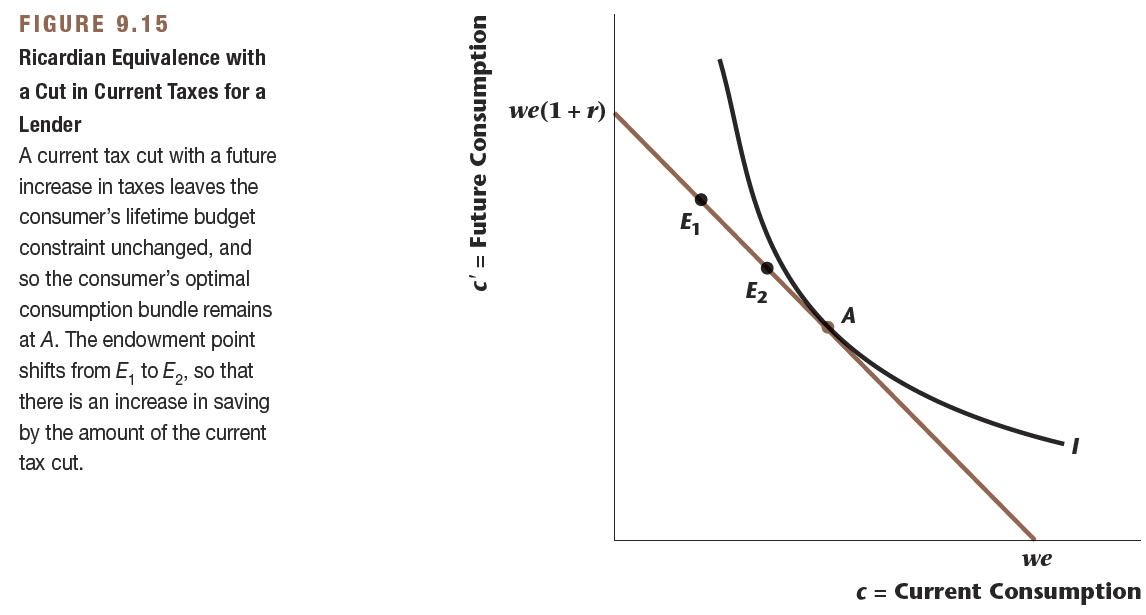
\includegraphics[width=0.8\linewidth]{figures/915}
		\end{figure*}
		
		\newpage
		\subsubsection{Credit Market}
		\begin{assumption}
			For $S^p(r)$, when $r$ changes, substitution effects out-weights the income effects when we add these effects across all consumers. (\emph{upward sloping private saving})
		\end{assumption}
		\par Ricardian Equivalence Theorem states that the change in tax scheme will not affect the real interest rate $r$. This means when there is a tax cut associated with an increase in $B$, consumers anticipates the future increase in tax. Then consumers increase $s$ and $S^p(r)$ for consumption smoothing. The supply in credit market increases so that the the equilibrium interest rate (i.e. $r^*\ s.t.\ S^p(r^*)=B $) is unchanged.
		
		\begin{figure*}
			\centering
			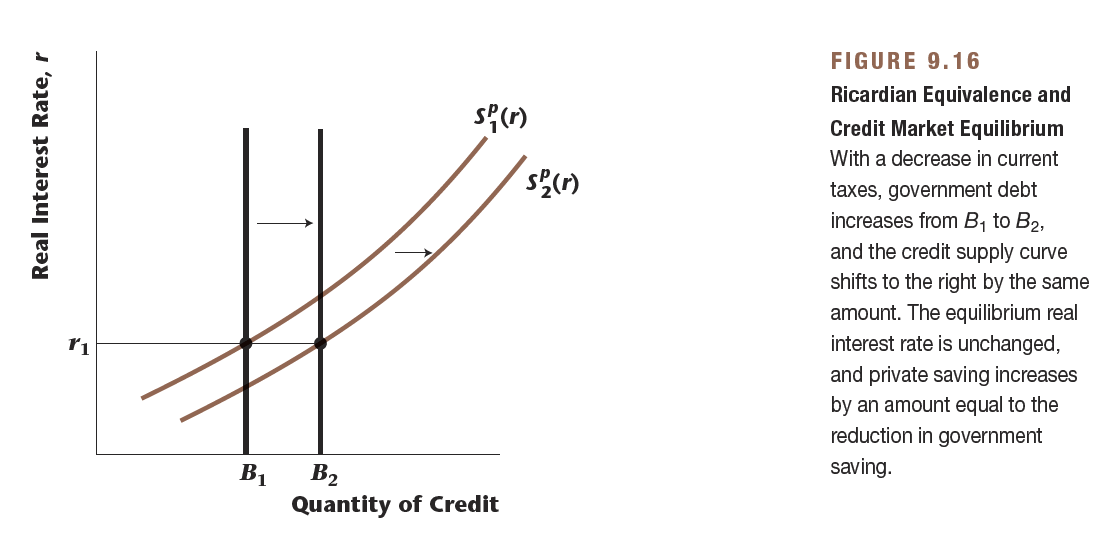
\includegraphics[width=0.8\linewidth]{figures/916}
		\end{figure*}
		
		
	\section{Chapter 11 A Real Inter-temporal Model with Investment}	
		\subsection{The Representative Consumer}
			\subsubsection{Setup}
			\paragraph{} Consumers are endowed with $h$ hours per period to allocate between working and leisure and non-labor income $\pi - T$ in each period.
			\par The representative consumer has \textbf{current period budget}
			\begin{equation}
				C + S^p = (h - l)w + \pi - T
			\end{equation}
			and \textbf{future period budget constraint} is
			\begin{equation}
				C' = (h - l')w' + (1+r)S^p + \pi' - T'
			\end{equation}
			The \textbf{life time present value constraint} is 
			\begin{equation}
				C + \frac{C'}{1+r} = (h - l)w + \pi - T + \frac{(h - l')w' + \pi' - T'}{1+r}
			\end{equation}
			
			\subsubsection{Optimization problem}
			\paragraph{} Given $w, w', T, T', \pi, \pi', r$, the representative consumer maximize his or her life time utility by choosing $C,C',l,l'$.
			\begin{multline}
				\\
				max_{C,C',l,l'} \big \{ \ln{C} + \eta \ln{l} + \beta \big [ \ln{C'} + \eta \ln{l'} \big] \big \} \\
				s.t.\ C + \frac{C'}{1+r} = (h - l)w + \pi - T + \frac{(h - l')w' + \pi' - T'}{1+r}
				\\
			\end{multline}
			\subsubsection{Optimal Solution}
			\paragraph{Solve} Solve above optimization problem with Lagrangian Multiplier method,
			\begin{equation}
				\mathcal{L} = \ln{C} + \eta \ln{l} + \beta[\ln{C'} + \eta \ln{l'}] + \lambda \big \{ w(h - l) + \pi - T + \frac{w'(h - l') + \pi' - T'}{1 + r} - C - \frac{C'}{1+r} \big \}
			\end{equation}
			the first order condition for optimal choice $(C^*, C'^*, l^*, l'^*)$ is
			\begin{equation}
				\begin{cases}
					\frac{\partial \mathcal{L}}{\partial C} = \frac{1}{C} - \lambda = 0 \\
					\frac{\partial \mathcal{L}}{\partial C'} = \frac{\beta}{C'} - \frac{\lambda}{1+r} = 0 \\
					\frac{\partial \mathcal{L}}{\partial l} = \frac{\eta}{l} - w\lambda = 0 \\
					\frac{\partial \mathcal{L}}{\partial l'} = \frac{\beta \eta}{l'} - \lambda \frac{w'}{1+r} = 0 \\
					\frac{\partial \mathcal{L}}{\partial \lambda} = w(h - l) + \pi - T + \frac{w'(h - l') + \pi' - T'}{1 + r} - C - \frac{C'}{1+r} = 0 \\
				\end{cases}
			\end{equation}
			\paragraph{Inter-temporal consumption}
			\begin{equation}
				\frac{1}{C} = (1+r)\frac{\beta}{C'}
			\end{equation}
			
			\paragraph{Inter-temporal leisure}
			\begin{equation}
				\frac{\beta \eta}{l'} = \frac{w'}{1+r} \frac{\eta}{w l}
			\end{equation}
			
			\paragraph{Intra-temporal leisure consumption}
			For current period
			\begin{equation}
				\frac{\eta}{l} = w \frac{1}{C}
			\end{equation}
			and for future period
			\begin{equation}
				\frac{\beta \eta}{l'} = \frac{\beta}{C'} w'
			\end{equation}
			
			\subsubsection{Current Labor Supply}
			\begin{assumption}
				The current labor supply satisfies the following assumptions.
				\begin{enumerate}
					\item The \underbar{quantity of} current labor supplied increases when the current real wage increases.
					\item Current labor supply increases when the real interest rate increases.
					\item Current labor supply decreases when lifetime wealth increases.
				\end{enumerate}				
			\end{assumption}
			
			\subsubsection{Current Demand for Consumption Goods}
			\paragraph{} Primary factors affecting current consumption are \underbar{lifetime wealth} and the \underbar{real interest rate}.
			
			\begin{definition}
				\textbf{Marginal propensity to consume} measures the amount that current consumption increases when there is a unit increase in aggregate real income.
			\end{definition}
				
			\begin{figure*}[h]
				\centering
				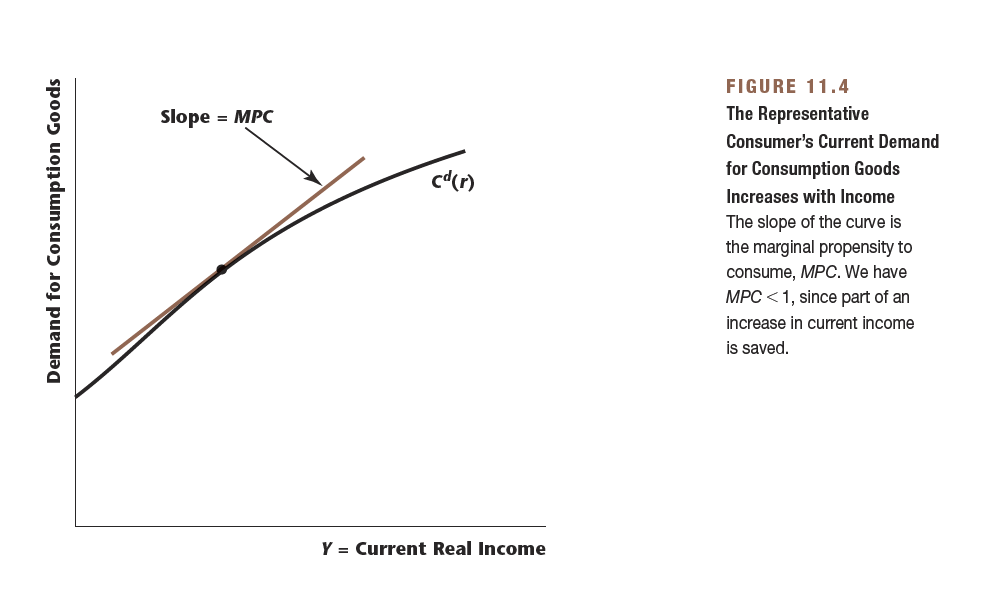
\includegraphics[width=\linewidth]{figures/114}
			\end{figure*}
			\newpage
			
			\begin{assumption}
				when interest rate change, for consumption scheme, the substitute effect dominates income effect.
			\end{assumption}
			\par Therefore, an increase in $r$ leads to a downward shifting of $C^d(r)$ as current period consumption becomes relatively more expensive.
			
			\subsection{The Representative Firm}
				\subsubsection{Optimization Problem}
				\paragraph{Setup} the firm want to maximize the \textbf{present value of lifetime profit} by choosing numbers of labor hired in each period and the investment, $(N,N',I)$ (equivalently, choosing $K'$).
				\paragraph{Production function}
					\begin{equation}
						Y = z F(K, N),\ Y' = z' F(K', N')
					\end{equation}
				\paragraph{Current period profit}
					\begin{equation}
						\pi = Y - wN - I
					\end{equation}
				\paragraph{Capital accumualtion}
					\begin{equation}
						K' = (1-d) K + I
					\end{equation}
				\paragraph{Future period profit} in future period, firm sales all its capital stock altogether with its output.
					\begin{equation}
						\pi' = Y' + (1-d)K' - wN'
					\end{equation}
				\paragraph{Present value for life time profit}
					\begin{equation}
						V = Y - wN + (1-d)K - K' + \frac{Y' + (1-d)K' - wN'}{1+r}
					\end{equation}
					
				\subsubsection{Optimal Solution}
					\paragraph{Labor choice} In both periods, the representative firm chooses $N, N'$ by equating the marginal revenue product(since price of output is normalized to 1, $MRP_N = MP_N$) and marginal cost ($w$) of labor. That's
					\begin{equation}
						\pd{zF(K, N)}{N} = MP_N = w
					\end{equation}
					\begin{equation}
						\pd{z'F{K', N'}}{N'} = MP_N' = w' 
					\end{equation}
					
					\paragraph{Investment schedule} Solving $\pd{V}{K'} = 0$ gives
					\begin{equation}
						1 = \frac{MP_K'+(1-d)}{1+r}
					\end{equation}
					rearrange the above equation,
					\begin{equation}
						r = MP_K' - d
					\end{equation}
					where the left hand side is the opportunity cost of investing one additional unit of $K'$ and the right hand side is the \textbf{net (of depreciation) marginal product of capital}.
					
					\begin{figure*}[h]
						\centering
						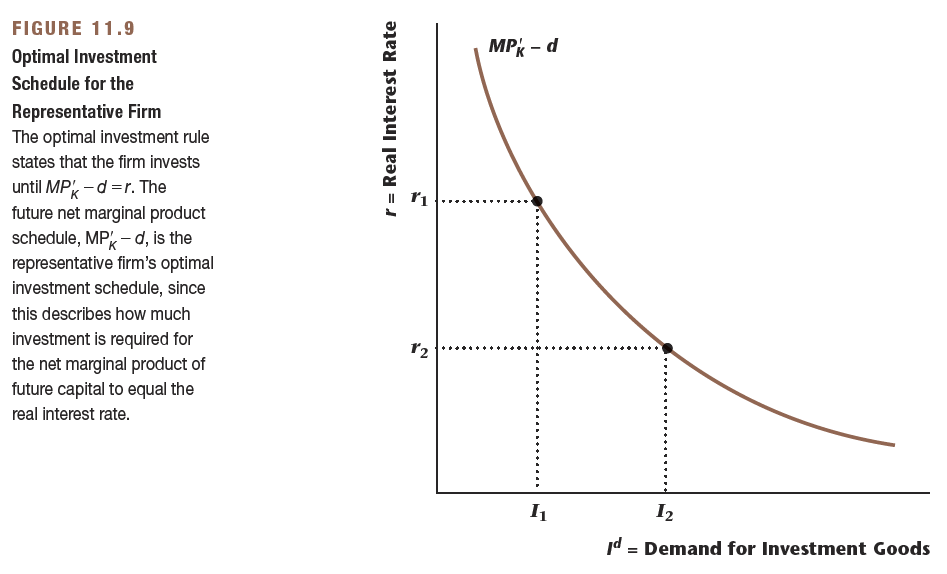
\includegraphics[width=\linewidth]{figures/119}
					\end{figure*}
					
					\paragraph{Change in optimal investment schedule} notice that we infer the optimal investment level by finding the optimal capital stock in the future period first.
					\begin{enumerate}
						\item The optimal investment schedule shifts to the right if future total factor productivity, $z'$, increases.
						\item The optimal investment schedule shifts to the left if initial capital endowment, $K$, increases.
					\end{enumerate}
			\subsection{Government}
				\paragraph{}Government sets government purchases of consumption goods exogenously in each period and have to satisfy its budget in terms of present discounted value.
				\begin{equation}
					G + \frac{G'}{1+r} = T + \frac{T'}{1+r}
				\end{equation}
				
			\subsection{Competitive Equilibrium}
				\subsubsection{The Current Labor Market and the Output Supply Curve}
					\paragraph{Steps}
						\begin{enumerate}
							\item Find labor market equilibrium $N^*$ by solving $N^s(w, r, \cdot) = N^d(w, \cdot)$
							\item Find equilibrium consumption good output using aggregate production function. $Y^* = zF(K, N^*)$
						\end{enumerate}
					\begin{figure*}[h]
						\begin{minipage}{0.5\linewidth}
						\centering
						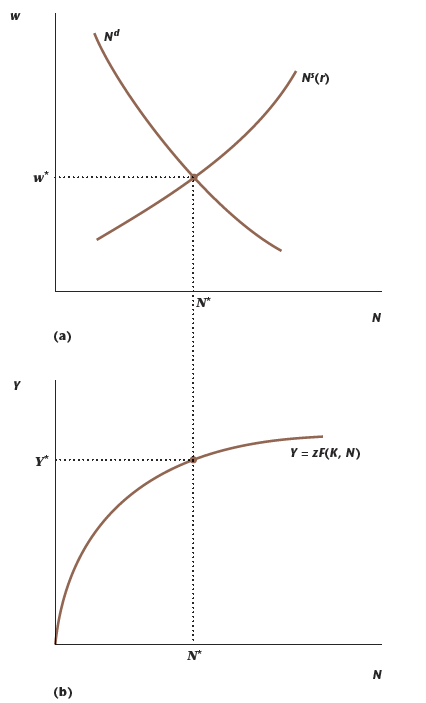
\includegraphics[width=\linewidth]{figures/1112}
						\end{minipage}
						\hfill
						\begin{minipage}{0.5\linewidth}
							\centering
							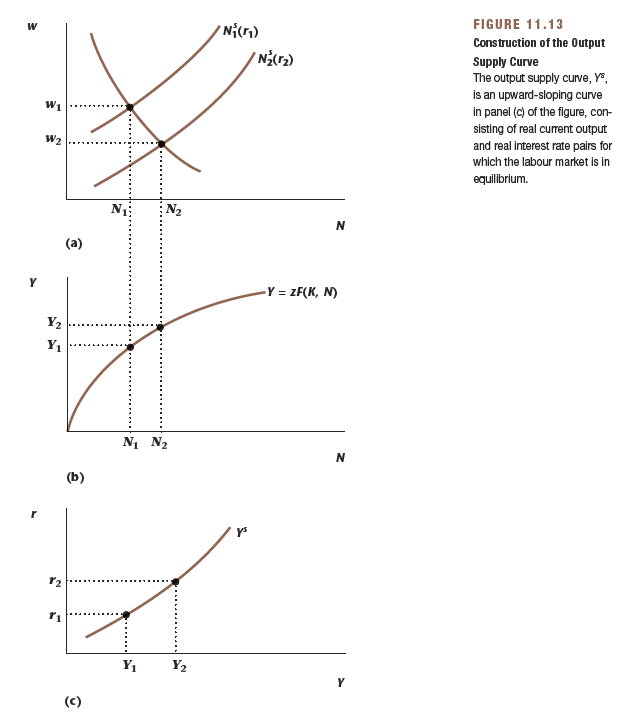
\includegraphics[width=1.4\linewidth]{figures/1113}
						\end{minipage}
						
					\end{figure*}
					
					\par Then we can construct the output supply curve $Y^s(r)$ as in figure 11.13.
					
				\newpage
				\subsubsection{Current Good Market and the Output Demand Curve}
				\paragraph{Steps} In a closed economy, the national income identity must hold,
					\begin{equation}
						Y = C^d(Y, r) + I^d(r) + G
					\end{equation}
					And $C^d(Y, r)$ depends on $Y$ as in figure 11.4, solving the equilibrium $Y^*$ by solving 
					\begin{equation}
						Y^*\ s.t.\ Y^* = C^d(Y^*,r) + I^d(r) + G
					\end{equation}
					\begin{figure*}[h]
						\centering
						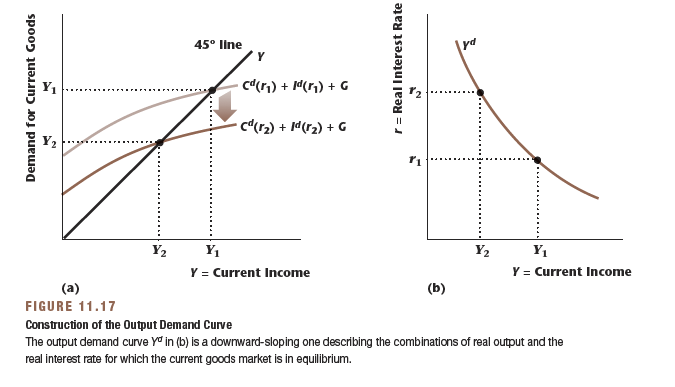
\includegraphics[width=\linewidth]{figures/1117}
					\end{figure*}
				
				\subsubsection{Credit Market}
					\paragraph{} By Walras' Law, as labor and consumption good markets clear, the credit market clears as a result.
				
				\subsubsection{Complete Model}
					\paragraph{} The complete general equilibrium model can be constructed as
					\begin{figure*}
						\centering
						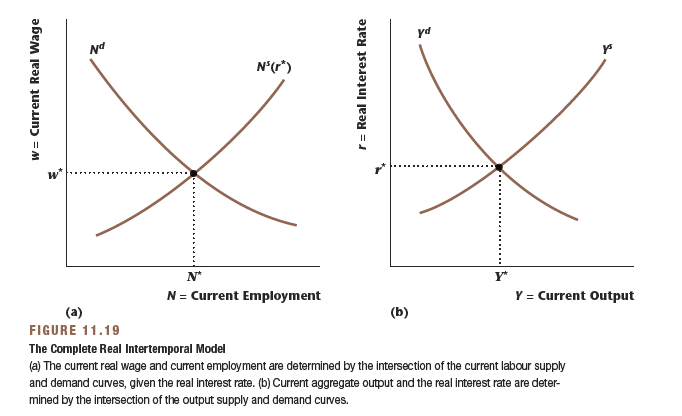
\includegraphics[width=0.7\linewidth]{figures/1119}
					\end{figure*}
				
			\subsection{Shocks to the General Equilibrium}
\end{document}




















